\documentclass[../../main/main.tex]{subfiles}
\begin{document}
\section{Game Value}
\label{sec:game_value}

LCP is a zero-sum game, so the value of the game can be found by the minimax theorem. Specifically, it is the maximum expected payoff that the bettor can gain when the caller plays optimally, and the minimum expected payoff that the caller can lose when the bettor plays optimally.

Since we have already found optimal strategies for both players, we can compute the value of the game as the average of the payoff in Nash equilibrium over all possible hand combinations $(x, y)$. This reduces to an integral of the payoff over the unit square, like we saw in Figure \ref{fig:payoffs}. Because the bet size is only defined implicitly in terms of the hand strength $x$, this is extremely nontrivial and requires breaking the square into regions based on the strategies and bet size. This method is fully specified in Appendix \ref{sec:value_computation}, but the resulting expression is given below.

\[
    V_{LCP}(L, U) = \frac{(1 + L)^3(1+U)^3 - ((1+L)^3+L^3(1 + U)^3)}{14(1 + L)^3(1+U)^3 - 2((1+L)^3+L^3(1 + U)^3)}
\]

This is a rational function of $L$ and $U$ with a surprisingly simple form.  Importantly, this makes it easy to compute $V_{LCP}(L, U)$ as $L, U$ approach their extreme values, which we use to relate the game value to that of NLCP and FBCP in the next section. 

Most interestingly, the value of LCP has the following symmetry:

\begin{align*}
    V_{LCP}(L, U) = V_{LCP}\left(\frac{1}{U}, \frac{1}{L}\right)
\end{align*}

This symmetry is easily checked from the definition of $V_{LCP}(L, U)$, but is not at all obvious from the game setup.

In the following sections, we investigate the properties and behavior of $V_{LCP}(L, U)$ in more detail. These include monotonicity, convergence to NLCP and FBCP, and the symmetry property.





\subsection{Value Monotonicity}

Intuitively, more options for the bettor should increase the game's value. To see this visually, we can plot the value of LCP as a function of the limits $L$ and $U$ for a range of values, as in Figure \ref{fig:payoffs_vs_LU_combined}.

\begin{figure}[h!]
    \begin{adjustwidth}{-1in}{-1in}
        \centering
        \begin{minipage}{0.6\textwidth}
            \centering
            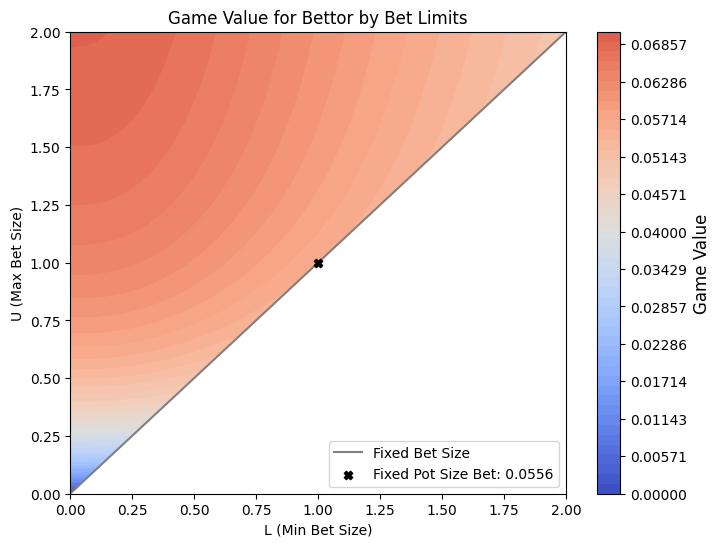
\includegraphics[width=\textwidth]{payoffs_by_limits.png}
            \caption*{(a) Linear scale}
        \end{minipage}
        \hspace{0.05\textwidth}
        \begin{minipage}{0.6\textwidth}
            \centering
            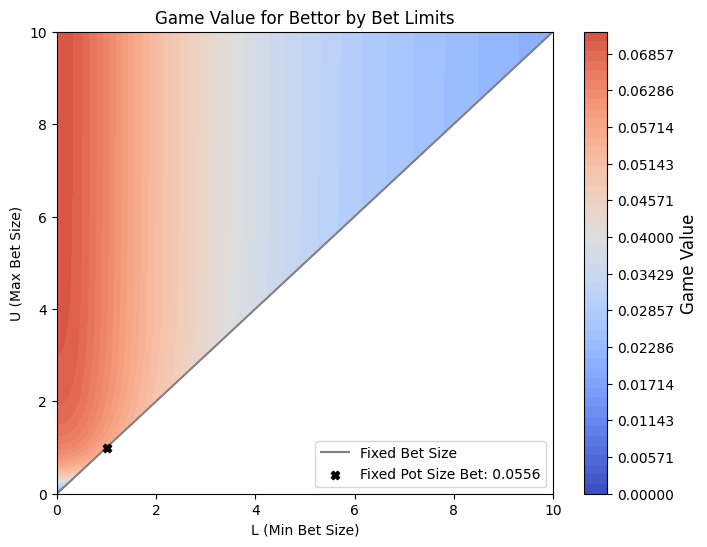
\includegraphics[width=\textwidth]{payoffs_by_limits_wide.png}
            \caption*{(b) Zoomed out linear scale}
        \end{minipage}
        \vspace{0.5cm}
        \begin{minipage}{0.6\textwidth}
            \centering
            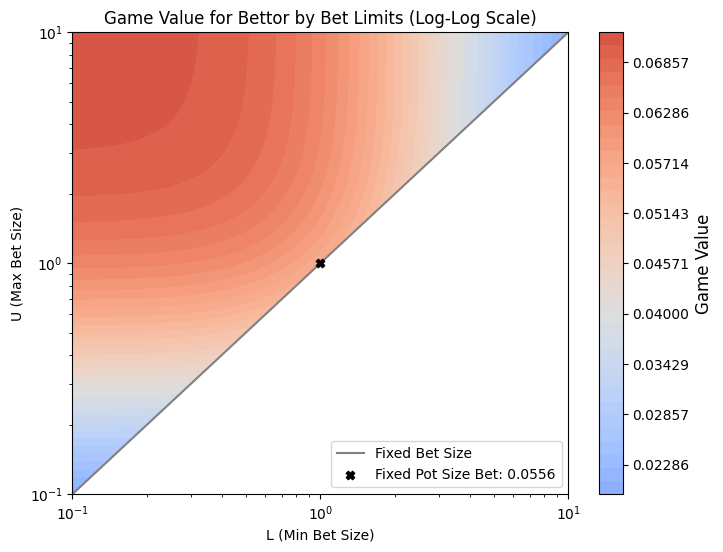
\includegraphics[width=\textwidth]{payoffs_by_limits_log.png}
            \caption*{(c) Log-log scale}
        \end{minipage}
        \hspace{0.05\textwidth}
        \begin{minipage}{0.6\textwidth}
            \centering
            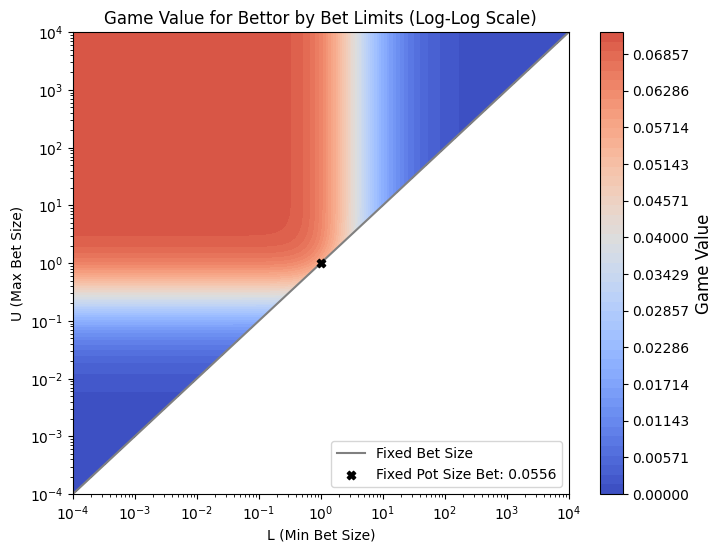
\includegraphics[width=\textwidth]{payoffs_by_limits_log_wide.png}
            \caption*{(d) Zoomed out log-log scale}
        \end{minipage}
    \end{adjustwidth}
    \caption{Game value of Limit Continuous Poker as a function of the limits $L$ and $U$. (a) Linear scale, (b) Zoomed out linear scale, (c) Log-log scale, (d) Zoomed out log-log scale. The restriction $L \leq U$ keeps the plots above the diagonal.}
    \label{fig:payoffs_vs_LU_combined}
\end{figure}

Notice the higher value for more lenient limits (top left of any plot in Figure \ref{fig:payoffs_vs_LU_combined}) and lower value for more strict limits (moving down/right). We can easily prove this formally:

\begin{theorem}
    The value of Limit Continuous Poker is monotonically increasing in $U$ and decreasing in $L$:
\[
    \frac{\partial V_{LCP}(L, U)}{\partial U} \geq 0, \;\; \frac{\partial V_{LCP}(L, U)}{\partial L} \leq 0
\]
\end{theorem}
\begin{customproof}
    \todo{prove this}
\end{customproof}

\subsection{Value Convergence}

The main diagonal of the plots in Figure \ref{fig:payoffs_vs_LU_combined} should represent $L=U$, which means the bet size is fixed. Thus, this diagonal should represent the value of FBCP for various values of $B$. We can prove this formally:

\begin{theorem}
    For any $B > 0$, the value of Limit Continuous Poker converges to the value of Fixed-Bet Continuous Poker as $L$ and $U$ approach $B$:
\[
\lim_{L \to B} \lim_{U \to B} V_{LCP}(L, U) = \lim_{U \to B} \lim_{L \to B} V_{LCP}(L, U) = V_{FB}(B)
\]
\end{theorem}

\begin{customproof}
    \todo{prove this}
\end{customproof}

These plots also align with the known result that a fixed pot-size bet of $B=1$ maximizes the expected value for the bettor in FBCP, as seen by the fact that $(1, 1)$ achieves the maximum value on the diagonal. 

We can also show that the value of LCP converges to the value of NLCP as $L$ and $U$ approach their extremes, represented by the top left of any plot in Figure \ref{fig:payoffs_vs_LU_combined}.

\begin{theorem}
    The value of Limit Continuous Poker converges to the value of NLCP as $L$ and $U$ approach $0$ and $\infty$:
\[
\lim_{L \to 0} \lim_{U \to \infty} V_{LCP}(L, U) = \lim_{U \to \infty} \lim_{L \to 0} V_{LCP}(L, U) = V_{NL}
\]
\end{theorem}
\begin{customproof}
    \todo{prove this}
\end{customproof}

\subsection{Value Symmetry}

Looking again at the log-log plots in Figure \ref{fig:payoffs_vs_LU_combined}, we see the symmetry property of $V_{LCP}(L, U)$ represented by symmetry about the reverse diagonal (the line $\log(L) = -\log(U)$). 

This symmetry can be interpreted in terms of how changing the limits affects the game to the bettor. We discussed earlier how the bettor benefits from increasing $U$ or from decreasing $L$, but it was unclear exactly how these benefits related quantitatively. The symmetry property tells us that the benefit from increasing $U$ is exactly equivalent to that of decreasing $L$ in a reciprocal manner, centered exactly around the pot size of $1$. Similarly, the loss in value from decreasing $U$ is equivalent to the loss from increasing $L$ in a reciprocal manner.

For example, suppose you are given the choice between playing LCP as the bettor with limits $L=1/2$ and $U=5$ or $L=1/5$ and $U=2$. You know you can play optimally, but it is unclear which game favors you. The symmetry property tells us that the value of the game is the same in both cases, so you should be indifferent between the two.

\end{document}